\newpage\section{Introduction} Isaac Asimov, the prolific American author, once wrote that \begin{quote} The most exciting phrase to hear [...], the one that heralds the most discoveries, is not ``Eureka!'' but ``That's funny...''.\end{quote}
However, anomalous observations are not only harbingers of great scientific discoveries -- unexpected observations can spoil analyses or be indicative of the presence of issues related to data collection or data processing. \par Either way, it becomes imperative for analysts and decision-makers to establish anomaly detection protocols, and to identify strategies to deal with such observations.  
\subsection{Basic Notions and Overview}
\textbf{Outlying observations} are data points which are \textbf{atypical} in comparison to the unit's remaining features (\textit{within-unit}), or in comparison to the measurements for other units (\textit{between-units}), or as part of a collective subset of observations. Outliers are thus observations which are \textbf{dissimilar to other cases} or which contradict \textbf{known dependencies} or rules.\footnote{Outlying observations may be anomalous along any of the individual variables, or in combination.}% (information in this section is taken partly from \cite{DP_OW,DP_A,DP_T,DP_CBK}).
\par Observations could be anomalous in one context, but not in another. Consider, for instance, an adult male who is 6-foot tall. Such a man would fall in the 86th percentile among Canadian males \cite{DP_HPC}, which, while on the tall side, is not unusual; in Bolivia, however, the same man would land in the 99.9th percentile \cite{DP_HPC}, which would mark him as extremely tall and quite dissimilar to the rest of the population.\footnote{Anomaly detection points towards interesting questions for analysts and subject matter experts: in this case, why is there such a large discrepancy in the two populations?}  
\begin{center}
    \rule{0.5\textwidth}{.4pt}
\end{center}
The most common mistake that analysts make when dealing with outlying observations is to remove them from the dataset without careful studying whether there are good reasons to retain them. \newl \textbf{Influential data points}, meanwhile, are observations whose absence leads to \textbf{markedly different} analysis results. When influential observations are identified, remedial measures (such as data transformation strategies) may need to be applied to minimize any undue effect. Note that outliers may be influential, and influential data points may be outliers, but the conditions are neither necessary nor sufficient. 
\paragraph{Detecting Anomalies}  Anomalies are by definition \textbf{infrequent}, and typically shrouded in \textbf{uncertainty} due to small (relative) sample sizes, which makes differentiating them from \textbf{noise} or \textbf{data entry errors} difficult. It could also be the case that the boundaries between a normal unit and a deviating unit is \textbf{fuzzy}; with the advent of e-shops, a purchase made at 3am local time does not necessarily ring alarm bells anymore. It is hard enough as it is to try to identify ``honest'' anomalies; when anomalies are associated with \textbf{malicious activities}, they are typically \textbf{disguised} to look like a normal observation, which muddies the picture even more. 
\newl
Numerous methods exist to identify anomalous observations; \textbf{none of them are foolproof} and judgement must be used. Methods that employ graphical aids (such as box-plots, scatterplots, scatterplot matrices, and 2D tours, for outliers, say \ref{sec:DV}) are particularly easy to implement and interpret, especially in a low-dimensional setting. Analytical methods also exist (using Cooke's or Mahalanobis' distances, say), but in general some additional level of analysis must be performed, especially when trying to identify influential points (\textit{cf.} \textbf{leverage}). 
\newl We do not recommend the general use of \textbf{automated detection/removal} -- as tempting as this might get when the dataset is large. This stems partly from the fact that that once the ``anomalous'' observations have been removed from the data set, previously ``regular'' observations can become anomalous in turn in the smaller dataset; it is not clear when the runaway train will stop.  \newl 
In the early stages, \textbf{simple data analyses} (such as descriptive statistics, 1- and 2-way tables, and  traditional visualisations) may be performed to help identify anomalous observations, or to obtain insights about the data, which could eventually lead to modifications of the analysis plan.
\paragraph{Outlier Tests} So how do we \textit{actually} detect outliers? Most methods come in one of two flavours: \textbf{supervised} and \textbf{unsupervised} (we will discuss those concepts -- and others -- in later sections).\newl 
Supervised methods use a historical record of \textbf{labeled} (that is to say, previously identified) anomalous observations to build a \textbf{predictive classification or regression model} which estimates the probability that a unit is anomalous; domain expertise is required to tag the data. Since anomalies are typically \textbf{infrequent}, these models often have to accommodate the rare occurrence problem (more on this in Section~\ref{sec:DSML}). Unsupervised methods, on the other hand, use no previous information or data; the following traditional methods and tests of outlier detection fall into this category (note that \textbf{normality} of the underlying data is an assumption for most tests; how robust these tests are against departures from this assumption depends on the situation).
\begin{center}
    \rule{0.5\textwidth}{.4pt}
\end{center}
Perhaps the most commonly known such test is \textbf{Tukey's boxplot test}: for normally distributed data, regular observations typically lie between the \textbf{inner fences} $$Q_1-1.5(Q_3-Q_1) \quad\mbox{and}\quad Q_3+1.5(Q_3-Q_1).$$ \textbf{Suspected outliers} lie between the inner fences and the \textbf{outer fences} 
$$Q_1-1.5(Q_3-Q_1) \quad\mbox{and}\quad Q_3+1.5(Q_3-Q_1).$$
Points beyond the outer fences are identified as \textbf{outliers} ($Q_1$ and $Q_3$ represent the data's   $1^{\textrm{st}}$ and $3^{\textrm{rd}}$ quartile, respectively; see Figure~\ref{fig:boxplot}).
\begin{figure}[t]
\centering
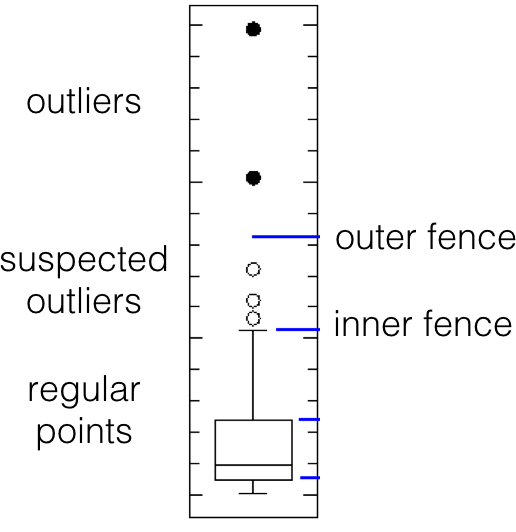
\includegraphics[width=0.30\textwidth]{Images/boxplot.png}
\caption[\small Tukey's boxplot test for outliers]{\small Tukey's boxplot test; suspected outliers are marked by white disks, outliers by black disks.}
\hrule\label{fig:boxplot}
\end{figure}
\afterpage{\FloatBarrier}
The \textbf{Grubbs test} is another univariate test, which takes into consideration the number of observations in the dataset. Let $x_i$ be the value of feature $X$ for the $i^{\textrm{th}}$ unit, $1\leq i\leq N$, $(\overline{x},s_x)$ be the mean and standard deviation of feature $X$, $\alpha$ be the significance level, and $T(\alpha,N)$ be the critical value of the Student $t$-distribution at significance $\alpha/2N$. Then, the $i^{\textrm{th}}$ unit is an \textbf{outlier along feature} $X$ if $$|x_i-\overline{x}| \geq \frac{s_x(N-1)}{\sqrt{N}}\sqrt{\frac{T^2(\alpha,N)}{N-2+T^2(\alpha,N)}}.$$
Other common tests include:
\begin{itemize}[noitemsep]
\item the \textbf{Dixon $Q$ test}, which is used in the experimental sciences to find outliers in (extremely) small datasets -- it is of dubious validity;
\item the \textbf{Mahalanobis distance}, which is linked to the leverage of an observation (a measure of influence), can also be used to find multi-dimensional outliers, when all relationships are linear (or nearly linear);
\item the \textbf{Tietjen-Moore} test, which is used to find a specific number of outliers;
\item the \textbf{generalized extreme studentized deviate}, if the number of outliers is unknown; 
\item the \textbf{chi-square} test, when outliers affect the foodneess-of-fit, as well as 
\item DBSCAN and other unsupervised outlier detection methods.
\end{itemize}
What do we do when the data is not normally distributed? We will discuss one possible approach after we present three more examples illustrating the basics of visual outlier and anomaly detection. 
\begin{center}
    \rule{0.5\textwidth}{.4pt}
\end{center}
On a specific day, the height of several plants in a nursery are measured. The records also show each plant's age (the number of days since the seed has been planted).    
\begin{figure*}[t]
\centering
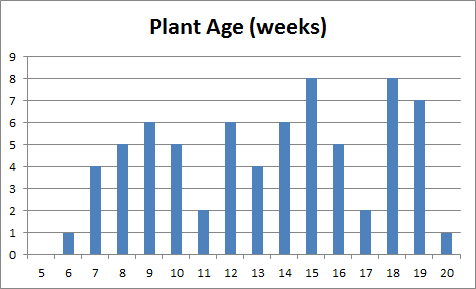
\includegraphics[width=0.32\textwidth]{Images/plant_age}\quad
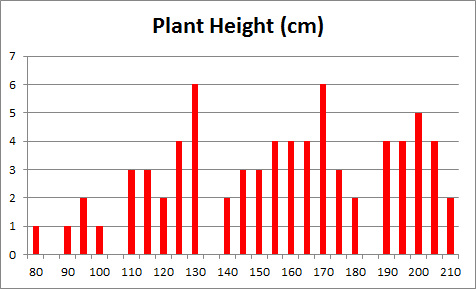
\includegraphics[width=0.32\textwidth]{Images/plant_height}\quad
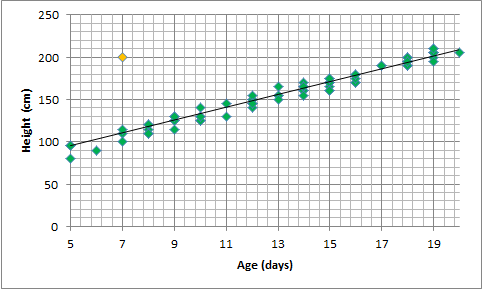
\includegraphics[width=0.32\textwidth]{Images/plant_height_vs_age}
\caption[\small Summary visualisations for a plant dataset]{\small Summary visualisations for an (artificial) plant dataset: age distribution (left), height distribution (middle), height vs. age, with linear trend (right).}\hrule \label{fig:plant_data}
\end{figure*}
Histograms of the data are shown in Figures~\ref{fig:planta} and \ref{fig:plantb}. Very little can be said about the data at that stage: the age of the plants (controlled by the nursery staff) seems to be somewhat haphazard, as does the response variable (height). A scatter plot of the data (see Figure~\ref{fig:plantc}), however, reveals that growth is strongly correlated with age during the early days of a plant's life for the observations in the dataset; most points clutter around a linear trend. But one point (in yellow) is easily identified as an \textbf{outlier}. There are at least two possibilities: either that measurement was botched or mis-entered in the database (representing an invalid entry), or that one specimen has experienced unusual growth (outlier). Either way, the analyst has to investigate further.  
\begin{center}
    \rule{0.5\textwidth}{.4pt}
\end{center}
A government department has 11 service points in a jurisdiction. Service statistics are recorded: in particular, the monthly average arrival rates per teller and monthly average service rates per teller for each service point are available. A scatter plot of the service rate per teller ($y$ axis) against the arrival rate per teller ($x$ axis), with linear regression trend, is shown in Figure~\ref{fig:servicea}. The trend is seen to inch upwards with increasing $x$ values. A similar graph, but with the left-most point removed from consideration, is shown in Figure~\ref{fig:serviceb}. The trend still slopes upward, but the fit is significantly improved suggesting that the removed observation is unduly \textbf{influential} -- a better understanding of the relationship between arrivals and services is afforded if it is set aside. Any attempt to fit that data point into the model must take that information into consideration. Note, however, that influential observations depend on the analysis that is ultimately being conducted -- a point may be influential for one analysis, but not for another.     
\begin{figure*}[t]
\centering
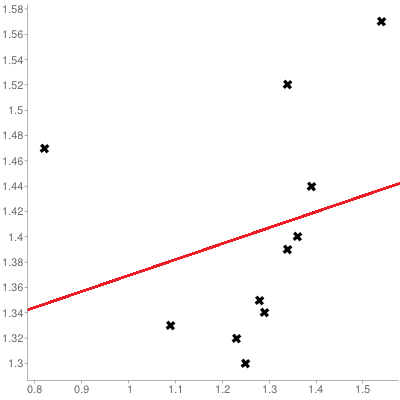
\includegraphics[width=0.32\textwidth]{Images/scatter_plot_linear_1}\quad
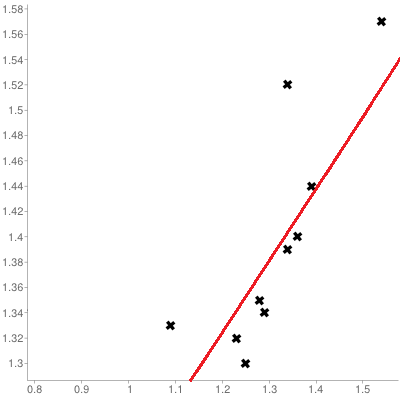
\includegraphics[width=0.32\textwidth]{Images/scatter_plot_linear_2}\quad
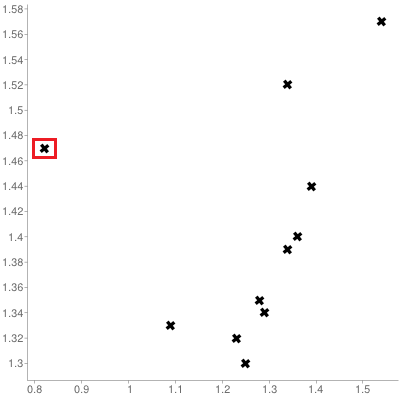
\includegraphics[width=0.32\textwidth]{Images/scatter_plot_2}
\caption[\small Visualisations for a service point dataset]{\small Visualisations for an (artificial) service point dataset: trend for 11 service points (left), trend for 10 service points (middle), influential observations (right).}\hrule
        \label{fig:service_data}
\end{figure*}
\begin{center}
    \rule{0.5\textwidth}{.4pt}
\end{center}
Measurements of the length of the appendage of a certain species of insect have been made on 71 individuals. Descriptive statistics have been computed; the results are shown in Figure~\ref{tab:appendagea}.
\begin{table*}[t]
\centering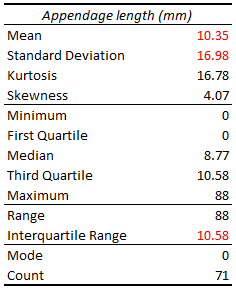
\includegraphics[width=0.26\textwidth]{{Images/appendage_length_descriptive}}\quad 
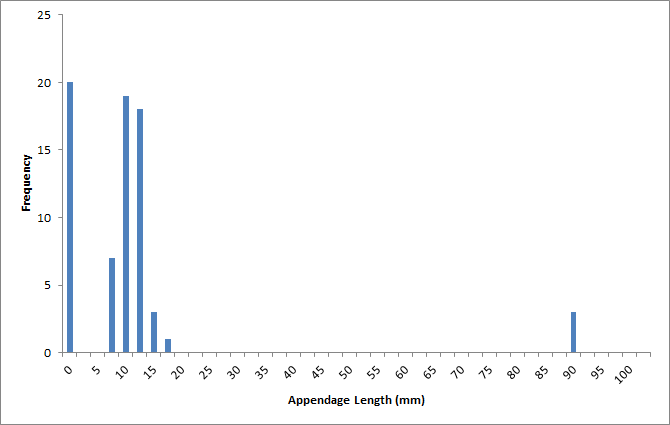
\includegraphics[width=0.50\textwidth]{{Images/appendage_length}}
\caption[\small Summary and visualisation for an appendage length dataset]{\small Summary and visualisation for an (artificial) appendage length dataset: descriptive statistics (left), appendge length distribution (right).}\hrule
\label{tab:appendage_data}
\end{table*}
Analysts who are well-versed in statistical methods would recognise the tell-tale signs that the distribution of appendage lengths is likely to be asymmetrical (since the skewness is non-negligible) and to have a ``fat'' tail (due to the kurtosis being commensurate with the mean and the standard deviation, the range being so much larger than the interquartile range, and the maximum value being so much larger than the third quartile). The mode, minimum, and first quartile values belong to individuals without appendages, so there would appear to be two sub-groups in the population (perhaps split along the lines of juveniles/adults, or males/females). The maximum value has already been seen to be quite large compared to the rest of the observations, which at first suggests that it might belong to an \textbf{outlier} or \textbf{invalid entry}. The histogram of the measurements, however, shows that there are 3 individuals with very long appendages (see Figure~\ref{tab:appendageb}): it now becomes plausible for these anomalous entries to belong to individuals from a different species altogether who were \textbf{erroneously added} to the dataset. This does not, of course, constitute a proof of such an error, but it raises the possibility, which is often the best that a consultant can do for a client.   

\subsection{Issues and Challenges}
jhvhjvhm
\subsection{Literature Review}
\subsection{Structure and Organization}
